% P11 project report. Build:  cd report && tectonic main.tex
\documentclass[12pt,a4paper]{report}

\usepackage[a4paper,left=1.25in,right=1in,top=1in,bottom=1in]{geometry}
\usepackage{amsmath}
\usepackage{graphicx}
\usepackage{booktabs}
\usepackage{tabularx}
\usepackage{array}
\usepackage{setspace}
\usepackage{xcolor}
\usepackage{listings}
\usepackage{float}
\usepackage{caption}
\usepackage{tikz}
\usetikzlibrary{arrows.meta,positioning,shapes.geometric}
\usepackage[hidelinks=false]{hyperref}
\hypersetup{citebordercolor={0 1 0}, linkbordercolor={1 0 0}, urlbordercolor={0 1 1}}

\graphicspath{{figures/}{../charts/}}
\setstretch{1.5}
\setlength{\parskip}{0.6em}
\setlength{\parindent}{0pt}
\setlength{\emergencystretch}{3em}  % fewer lines sticking out into the margin
\captionsetup{font=small}

\lstset{basicstyle=\ttfamily\footnotesize, breaklines=true, frame=single,
        columns=fullflexible, keepspaces=true, showstringspaces=false}

% ---------------------------------------------------------------------------
% Details to fill in. Anything in red still needs a real value.
% ---------------------------------------------------------------------------
\newcommand{\todo}[1]{\textcolor{red}{#1}}
\newcommand{\projtitle}{Electricity Load and Renewable Energy in Europe: A Hadoop-Based Analysis}
\newcommand{\guide}{\todo{[Guide name]}}
\newcommand{\coordinator}{\todo{[Course coordinator]}}
\newcommand{\hod}{Dr. Pramod Ganjewar}
\newcommand{\yearname}{\todo{[FOURTH]} YEAR BACHELOR OF TECHNOLOGY}
\newcommand{\acadyear}{\todo{2026--2027}}
\newcommand{\semester}{\todo{VII}}
\newcommand{\course}{Big Data Analytics}
\newcommand{\members}{%
  \begin{tabular}{@{}p{6cm}l@{}}
  \textbf{Krishna Mungase}   & \textbf{(Exam Seat No. 202301040029)}\\[4pt]
  \textbf{Sakshi Deshmukh}   & \textbf{(Exam Seat No. \todo{[seat no.]})}\\[4pt]
  \textbf{Vaishnavi Bhosale} & \textbf{(Exam Seat No. 202301040118)}\\[4pt]
  \textbf{\todo{[Sneh full name]}} & \textbf{(Exam Seat No. \todo{[seat no.]})}
  \end{tabular}}

\renewcommand{\bibname}{References}

\begin{document}

% =========================== Title page ===================================
\begin{titlepage}
\centering\setstretch{1.15}
\vspace*{-1.2cm}\rule{\textwidth}{0.4pt}\\[0.6cm]

\includegraphics[width=0.45\textwidth]{mitaoe_logo.png}\\[0.8cm]
{\large\bfseries A Project Report on}\\[0.5cm]
{\Large\bfseries \projtitle}\\[0.5cm]
{\itshape\bfseries Submitted by,}\\[0.3cm]
\members\\[0.5cm]
{\itshape\bfseries Guided by,}\\[0.2cm]
{\large\bfseries \guide}\\[0.6cm]
{\bfseries A Report submitted to MIT Academy of Engineering, Alandi(D), Pune,\\
An Autonomous Institute Affiliated to Savitribai Phule Pune University\\
in partial fulfillment of the requirements of the course \course\ in}\\[0.5cm]
{\bfseries \yearname}\\[0.1cm]
{\large\bfseries Computer Engineering}\\[0.5cm]
{\large\bfseries Department of Computer Engineering}\\[0.1cm]
{\Large\bfseries MIT Academy of Engineering}\\
(An Autonomous Institute Affiliated to Savitribai Phule Pune University)\\
{\large\bfseries Alandi (D), Pune -- 412105}\\[0.3cm]
{\Large\bfseries (\acadyear)}\\[0.3cm]
\rule{\textwidth}{0.4pt}
\end{titlepage}

% =========================== Certificate ==================================
\thispagestyle{empty}
\begin{center}

\includegraphics[width=0.45\textwidth]{mitaoe_logo.png}\\[1.2cm]
{\Large\bfseries\underline{CERTIFICATE}}
\end{center}
\vspace{0.5cm}
It is hereby certified that the work which is being presented in the \course\ project report entitled \textbf{``\projtitle''}, in partial fulfillment of the requirements of the course \course\ of the Bachelor of Technology in Computer Engineering and submitted to the \textbf{Department of Computer Engineering} of \textbf{MIT Academy of Engineering, Alandi(D), Pune, Affiliated to Savitribai Phule Pune University (SPPU), Pune}, is an authentic record of work carried out during Academic Year \textbf{\acadyear} Semester \textbf{\semester}, under the supervision of \textbf{\guide}, \textbf{Department of Computer Engineering}.

\vspace{1cm}
\begin{center}\members\end{center}
\vspace{1.5cm}
\begin{tabular*}{\textwidth}{@{\extracolsep{\fill}}cc}
\textbf{\guide} & \textbf{\hod}\\
\textbf{Course Teacher} & \textbf{HoD}
\end{tabular*}
\clearpage

% =========================== Declaration ==================================
\thispagestyle{empty}
\begin{center}{\Large\bfseries\underline{DECLARATION}}\end{center}
\vspace{0.4cm}
We the undersigned solemnly declare that the project report is based on our own work carried out during the course of our study under the supervision of \textbf{\guide}.

We assert the statements made and conclusions drawn are an outcome of our project work. We further certify that
\begin{enumerate}
\item The work contained in the report is original and has been done by us under the general supervision of our supervisor.
\item The work has not been submitted to any other Institution for any other degree/diploma/certificate in this Institute/University or any other Institute/University of India or abroad.
\item We have followed the guidelines provided by the Institute in writing the report.
\item Whenever we have used materials (data, theoretical analysis, and text) from other sources, we have given due credit to them in the text of the report and giving their details in the references.
\end{enumerate}
\vspace{1cm}
\begin{center}\members\end{center}
\clearpage

\pagenumbering{roman}
\setcounter{page}{4}

% =========================== Abstract =====================================
\chapter*{Abstract}
\addcontentsline{toc}{chapter}{Abstract}
Electricity grids in Europe now take a growing share of their power from wind and solar, which do not follow demand the way a power station can. This project studies six years of hourly data (January 2015 to September 2020) on electricity load, solar generation and wind generation for ten European countries, taken from the Open Power System Data time series package \cite{opsd2020,wiese2019}. The aim was to answer five questions a grid operator would ask, and to do it with the Hadoop tools covered in the course.

The 130 MB source file was reshaped from 300 columns into 1,480,855 readings and stored in HDFS on a single-node, pseudo-distributed Hadoop 3.4.2 cluster. Two MapReduce jobs written in Java compute average load per country-year and renewable share per country-month, using a combiner, a custom partitioner and custom counters; the combiner cut the data sent to the reducers from 12.9 MB to 1.5 KB. A Pig script finds peak load hours and daily generation, and Hive 4.2.1 holds external, managed, partitioned, Parquet and ORC tables and runs the analysis queries, including a join with grouping and the window functions RANK and LAG. The Parquet and ORC copies were 6.4 and 9.5 times smaller than the CSV.

Denmark had the highest renewable share in every year, rising from 43\% to 50\% of load between 2015 and 2019, and Germany grew the most, from 23\% to 34\%. Wind matches demand by season but not within the day, the biggest load changes happen in the morning ramp between 06:00 and 08:00, and hourly solar output is only weakly related to load (correlation 0.12 to 0.36). Along the way we found and removed 70 faulty readings in the source data, which Pig and Hive outputs exposed.

\textbf{Keywords:} Hadoop, HDFS, MapReduce, Pig, Hive, Parquet, renewable energy, electricity load

% =========================== Acknowledgment ===============================
\chapter*{Acknowledgment}
\addcontentsline{toc}{chapter}{Acknowledgment}
We thank our course teacher, \guide, for teaching the Big Data Analytics course and for the guidance during this project. The lab sessions on HDFS and the combiner experiment in CE-03 were the starting point for much of this work.

We thank \hod, Head of the Department of Computer Engineering, and the faculty of the department for the lab facilities and support.

We also thank the Open Power System Data project for publishing clean, well-documented electricity data under an open licence, and the Apache Hadoop, Pig and Hive communities for the software we used.

\tableofcontents
\listoffigures
\listoftables

\clearpage
\pagenumbering{arabic}

% ==========================================================================
\chapter{Introduction}

\section{Background}
An electricity grid has to match supply and demand every second. For most of the last century the supply side was made of power stations that could be scheduled: coal, gas, nuclear and hydro. Wind turbines and solar panels are different. They produce when the wind blows and the sun shines, and the grid operator can only forecast them, not order them. As their share grows, operators need to know how renewable output and demand move over the day and over the year, and where they do not line up.

The European grid operators publish hourly load and generation data on the ENTSO-E Transparency Platform \cite{entsoe}. The Open Power System Data (OPSD) project collects this data, checks it, and publishes it as one table per time resolution \cite{opsd2020,wiese2019}. Its hourly file has one row per hour from 2015 to 2020 and about 300 columns, one per country and measurement.

\section{Motivation}
The data is not large by industry standards (130 MB), but it has the shape of a typical big data problem: many records, a wide schema, gaps and errors in the source, and questions that need grouping, joining and windowed comparisons across millions of rows. That makes it a good case for practising the Hadoop stack end to end, from storing files in HDFS to querying them with SQL, with results small enough to check by hand.

\section{Problem statement}
A grid operator wants to understand demand and solar and wind output in ten European countries. Using HDFS, MapReduce, Pig and Hive, answer:
\begin{enumerate}
\item Which country has the highest renewable share, and how has it changed over the years?
\item What does the daily load curve look like in summer and in winter?
\item When does wind generation peak, and does that line up with demand?
\item Which hours show the largest changes in load?
\item How strongly is solar generation related to load?
\end{enumerate}
Renewable share is defined as (solar + wind) / load.

\section{Objectives}
\begin{enumerate}
\item Set up Hadoop in pseudo-distributed mode with Pig and Hive on our own machine.
\item Store the data in HDFS and demonstrate directories, block size, replication and \texttt{fsck}.
\item Write at least two MapReduce jobs in Java with a combiner, a partitioner and custom counters.
\item Use at least six Pig operators and Hive external, managed, partitioned and Parquet/ORC tables, including a join with grouping and aggregation.
\item Draw at least three charts from Pig and Hive output.
\item Run the same jobs on a sample and on the full data and compare time and counters.
\end{enumerate}

\section{Report organization}
Chapter~\ref{ch:lit} summarises the tools and the dataset. Chapter~\ref{ch:data} describes the data and how it was cleaned. Chapter~\ref{ch:setup} covers the cluster setup and the overall pipeline. Chapter~\ref{ch:impl} explains the HDFS, MapReduce, Pig and Hive work. Chapter~\ref{ch:results} answers the five questions and reports the scale test. Chapter~\ref{ch:problems} lists the problems we met, and Chapter~\ref{ch:concl} concludes. All code, outputs and step-by-step documentation are in our repository \cite{repo}.

% ==========================================================================
\chapter{Literature Review}\label{ch:lit}

\section{Distributed storage and processing}
The Google File System \cite{gfs2003} showed that a cluster of cheap machines can store very large files reliably by splitting them into large blocks and keeping several copies of each block on different machines. HDFS follows the same design \cite{hdfs2010}: a NameNode keeps the file system metadata (which blocks make up a file and where they are), and DataNodes store the blocks, 128 MB each by default, with three copies by default.

MapReduce \cite{dean2008} is a programming model for processing such files in parallel. A map function turns each input record into key-value pairs; the framework groups all values by key (the shuffle) and a reduce function combines the values of each key. An optional combiner runs the reduce logic on the map side to shrink the data before the shuffle. Lin and Dyer point out that this is only correct when the operation can be applied in parts, which rules out computing an average directly; the standard fix is to pass sums and counts \cite{lin2010}. In Hadoop 2 and later, YARN separates resource management from MapReduce, so that a ResourceManager hands out containers to any framework \cite{yarn2013}. White's book is the standard reference for configuring and running all of these \cite{white2015}.

\section{Higher-level languages}
Writing every analysis as Java MapReduce is slow. Pig Latin \cite{olston2008} describes a data flow as a sequence of steps (LOAD, FILTER, GROUP, JOIN, STORE) and compiles it into MapReduce jobs, optimising across steps. Hive \cite{thusoo2009} goes further and offers SQL over files in HDFS, with table definitions kept in a metastore. Later Hive versions added the ORC columnar format, vectorised execution and window functions \cite{huai2014}.

\section{Columnar storage}
Row formats such as CSV must be read in full even when a query needs two columns. Columnar formats store each column together, so a query reads only the columns it uses, and similar values compress well. Dremel introduced the nested columnar layout \cite{melnik2010} on which Apache Parquet is based \cite{parquet}; ORC is the columnar format developed for Hive \cite{huai2014}.

\section{The dataset}
The OPSD time series package \cite{opsd2020} contains load, wind and solar generation, capacity and prices for European countries at 15, 30 and 60 minute resolution, collected mainly from the ENTSO-E Transparency Platform \cite{entsoe}. Wiese et al. describe how the project collects, checks and documents the data, and note that the source data contains gaps and outliers that users should check for \cite{wiese2019}. We found such errors ourselves (Chapter~\ref{ch:data}).

% ==========================================================================
\chapter{Dataset and Data Preparation}\label{ch:data}

\section{Source}
We used the file \texttt{time\_series\_60min\_singleindex.csv}, version 2020-10-06 \cite{opsd2020}: 130,339,665 bytes, 50,401 hourly rows and 300 columns, from 2014-12-31 23:00 to 2020-09-30 23:00 UTC. For each country we took three columns: actual load, solar generation and wind generation, all in MW.

\section{Choosing the countries}
The plan named Germany, France, Spain, Italy, the Netherlands, Belgium, Austria, Denmark, Poland and Portugal. Before using them we measured, for each column, how many hours have a value and whether the yearly averages are believable. Table~\ref{tab:swap} lists what we changed.

\begin{table}[H]
\centering\small
\caption{Changes to the country list after checking the data}\label{tab:swap}
\begin{tabularx}{\textwidth}{lXX}
\toprule
Country & Problem found & Action\\
\midrule
Poland & solar column empty for 92\% of hours & replaced by Czech Republic (load, solar and wind about 100\% filled)\\
Netherlands & solar averages 364 MW in 2018, then 1 MW in 2019; wind also falls & replaced by Greece (100\% filled in every year)\\
Italy & 2015: wind almost entirely empty, solar 75\% empty & 2015 dropped; Italy starts in 2016\\
Portugal & offshore wind column only starts in June 2020 & empty offshore cells before that counted as 0 MW\\
\bottomrule
\end{tabularx}
\end{table}

The final list is Germany (DE), France (FR), Spain (ES), Italy (IT), Greece (GR), Belgium (BE), Austria (AT), Denmark (DK), Czech Republic (CZ) and Portugal (PT). Where a country has no total wind column we used onshore plus offshore.

\section{Wide to long}
The source has one row per hour and one column per country and metric. We converted it to one line per reading, without a header, so that every line has the same four fields and can be parsed the same way by MapReduce, Pig and Hive:
\begin{lstlisting}
2019-01-01 00:00:00,DE,load,43120.50
2019-01-01 00:00:00,DE,solar,0.00
2019-01-01 00:00:00,DE,wind,21340.00
\end{lstlisting}
Empty cells were dropped rather than written as zero, since an unknown reading is not a zero reading. The script \texttt{prep/reshape.py} writes the full file (1,480,855 lines, 52.9 MB) and a 2019-only sample (262,011 lines, 9.4 MB).

\section{Removing faulty readings}
Two later steps showed readings that cannot be real. Pig's peak-hour output (Section~\ref{sec:pig}) showed France at 158,000 MW for one hour on 2020-07-07, between hours of about 48,000 MW; France's highest real hour in the data is 94,492 MW. Hive's hourly-change query (Section~\ref{sec:hive}) was topped by Spanish hours where load fell by a third and came back the next hour, and Austria had whole days at about a quarter of normal load. We added four rules to \texttt{reshape.py}:
\begin{itemize}
\item spike: more than 25\% above the 99.9th percentile of that country and metric and more than 30\% above the median of the 7 surrounding hours (all metrics);
\item short dip: load below 70\% of the 7-hour median;
\item long dip: load below 50\% of the 25-hour median;
\item bad day: a day whose average load is below 50\% of the country's normal day.
\end{itemize}
They removed 70 readings: 10 spikes (France and Denmark), 5 short dips (Spain and Denmark), 7 night hours and 2 whole days in Austria in 2015. Before settling on the 50\% limit for days we tried 60\%, which flagged Italian Easter days and the April 2020 lockdown Sundays; those are real, so the limit was lowered.

% ==========================================================================
\chapter{System Setup and Methodology}\label{ch:setup}

\section{Hardware and software}
\begin{table}[H]
\centering\small
\caption{Environment}\label{tab:env}
\begin{tabularx}{\textwidth}{lX}
\toprule
Item & Version / value\\
\midrule
Machine & Apple MacBook Air (Apple Silicon, arm64), 8 GB RAM\\
Operating system & macOS 27.0.1\\
Java & OpenJDK 21.0.8\\
Hadoop (HDFS, YARN, MapReduce) & 3.4.2, pseudo-distributed\\
Apache Pig & 0.18.0\\
Apache Hive & 4.2.1, embedded Derby metastore, MapReduce engine\\
Build tool for Java jobs & Maven 3.9.9\\
Python (preparation, charts) & 3.14 with pandas 3.1.1, matplotlib 3.11.2\\
\bottomrule
\end{tabularx}
\end{table}

In pseudo-distributed mode every Hadoop daemon (NameNode, DataNode, ResourceManager, NodeManager, JobHistoryServer) runs as a separate process on one machine, so jobs go through the same steps as on a real cluster. Our configuration follows the Hadoop documentation \cite{hadoopdocs} and is kept in the project (\texttt{setup/hadoop-conf}) instead of the Hadoop install folder. Replication is set to 1, since there is one DataNode, and YARN may use 4 GB of memory.

\section{Pipeline}
Figure~\ref{fig:pipeline} shows the flow of data through the project.

\begin{figure}[H]
\centering
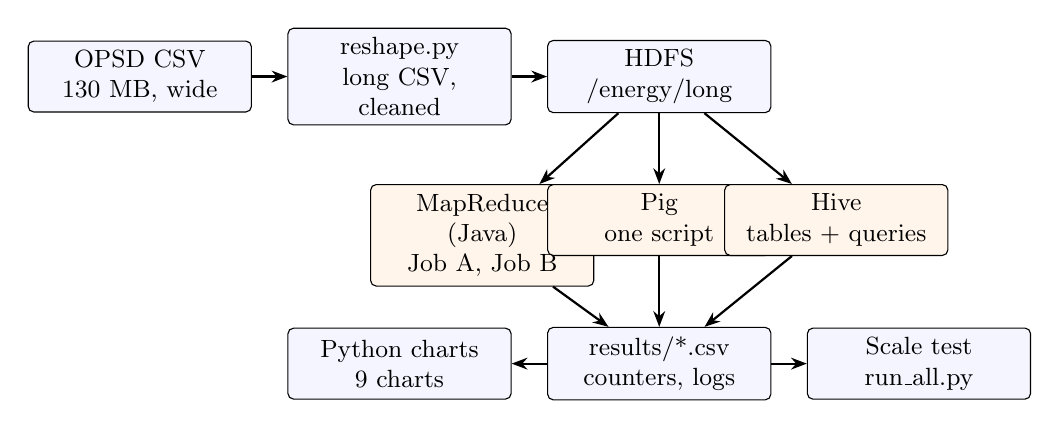
\begin{tikzpicture}[node distance=0.55cm and 0.45cm, every node/.style={font=\small},
  box/.style={draw, rounded corners=2pt, align=center, minimum height=0.9cm, text width=2.6cm, fill=blue!4},
  tool/.style={draw, rounded corners=2pt, align=center, minimum height=0.9cm, text width=2.6cm, fill=orange!8},
  arr/.style={-{Stealth[length=2mm]}, thick}]
\node[box] (raw) {OPSD CSV\\130 MB, wide};
\node[box, right=of raw] (prep) {reshape.py\\long CSV, cleaned};
\node[box, right=of prep] (hdfs) {HDFS\\/energy/long};
\node[tool, below left=0.9cm and -0.6cm of hdfs] (mr) {MapReduce (Java)\\Job A, Job B};
\node[tool, below=0.9cm of hdfs] (pig) {Pig\\one script};
\node[tool, below right=0.9cm and -0.6cm of hdfs] (hive) {Hive\\tables + queries};
\node[box, below=0.9cm of pig] (res) {results/*.csv\\counters, logs};
\node[box, left=of res] (ch) {Python charts\\9 charts};
\node[box, right=of res] (scale) {Scale test\\run\_all.py};
\draw[arr] (raw) -- (prep); \draw[arr] (prep) -- (hdfs);
\draw[arr] (hdfs) -- (mr); \draw[arr] (hdfs) -- (pig); \draw[arr] (hdfs) -- (hive);
\draw[arr] (mr) -- (res); \draw[arr] (pig) -- (res); \draw[arr] (hive) -- (res);
\draw[arr] (res) -- (ch); \draw[arr] (res) -- (scale);
\end{tikzpicture}
\caption{Data flow of the project}\label{fig:pipeline}
\end{figure}

\section{Team contributions}
\begin{table}[H]
\centering\small
\caption{Work split}\label{tab:team}
\begin{tabularx}{\textwidth}{lX}
\toprule
Member & Work\\
\midrule
Krishna Mungase & Hadoop, Pig and Hive setup; data preparation and cleaning; HDFS; scale test\\
Sakshi Deshmukh & Java MapReduce jobs, combiner, partitioner, counters\\
Vaishnavi Bhosale & Pig script; Hive tables, Parquet/ORC and analysis queries\\
\todo{[Sneh full name]} & Charts, findings, report and slides\\
\bottomrule
\end{tabularx}
\end{table}

% ==========================================================================
\chapter{Implementation}\label{ch:impl}

\section{HDFS}
We created six directories under \texttt{/energy}: \texttt{raw}, \texttt{long/sample}, \texttt{long/full}, \texttt{long/full\_32mb}, \texttt{output} and \texttt{warehouse}, and uploaded the raw and long files. The full long file was uploaded a second time with a 32 MB block size:
\begin{lstlisting}
hdfs dfs -D dfs.blocksize=33554432 -put energy_full.csv /energy/long/full_32mb/
\end{lstlisting} \texttt{hdfs fsck} confirms the difference (Table~\ref{tab:blocks}).

\begin{table}[H]
\centering\small
\caption{Block layout reported by \texttt{fsck}}\label{tab:blocks}
\begin{tabularx}{\textwidth}{Xrrl}
\toprule
File (under /energy) & Size (bytes) & Block size & Blocks\\
\midrule
long/full & 52,895,430 & 128 MB & 1\\
long/full\_32mb & 52,895,430 & 32 MB & 2 (33,554,432 + 19,340,998)\\
raw (original wide file) & 130,339,665 & 128 MB & 1\\
\bottomrule
\end{tabularx}
\end{table}

The raw file looks larger than 128 MB but is not: 128 MB here is $128 \times 1024^2 = 134{,}217{,}728$ bytes. We then raised the replication of the sample file to 2 with \texttt{hdfs dfs -setrep 2}. \texttt{fsck} reported \emph{``Target Replicas is 2 but found 1 live replica''} and one under-replicated block, while the status stayed HEALTHY. HDFS never places two copies of a block on the same DataNode, and we have only one, so the second copy cannot be made; no data is lost. We did not use \texttt{-setrep -w}, which waits for the copies and would never return here.

\section{MapReduce}
Both jobs are in one Maven project and read the long CSV.

\textbf{Job A (average load per country per year).} The mapper keeps load readings and emits the key \texttt{country,year} with a \texttt{SumCountWritable} value (sum, count). The combiner adds sums and counts but never divides; the reducer adds them and divides once. Dividing in the combiner would give averages of averages, which are wrong when groups differ in size \cite{lin2010}.

\textbf{Job B (renewable share per country per month).} The mapper puts each reading into the solar, wind or load slot of an \texttt{EnergySumsWritable}, which also counts hours per metric; the combiner adds the slots. The reducer computes
\[ \text{share} = \frac{\overline{\text{solar}} + \overline{\text{wind}}}{\overline{\text{load}}} \]
where each mean is taken over the hours that metric has data for. Belgian wind is missing in 5 to 25\% of hours each month while load is complete; dividing plain totals would count those hours as zero wind (12.8\% instead of 13.6\% for July 2019).

\textbf{Partitioner and counters.} \texttt{CountryPartitioner} hashes only the country part of the key, so every key of a country goes to the same reducer and each output file holds whole countries. With 3 reducers the split was BE and GR; CZ and IT; and the other six countries, which matches a hand calculation of \texttt{hashCode() mod 3}. Custom counters record bad lines and records per metric; a test file with four broken lines gave \texttt{BAD\_LINES=4}.

\begin{table}[H]
\centering\small
\caption{MapReduce counters on the full data, combiner on and off (3 reducers)}\label{tab:mr}
\begin{tabular}{lrrrr}
\toprule
& \multicolumn{2}{c}{Job A} & \multicolumn{2}{c}{Job B}\\
Counter & combiner & none & combiner & none\\
\midrule
Map input records & 1,480,855 & 1,480,855 & 1,480,855 & 1,480,855\\
Map output records & 494,920 & 494,920 & 1,480,855 & 1,480,855\\
Combine output records & 59 & -- & 688 & --\\
Reduce input records & 59 & 494,920 & 688 & 1,480,855\\
Reduce shuffle bytes & 1,552 & 12,867,938 & 41,986 & 90,332,173\\
Wall-clock time (s) & 21 & 24 & 24 & 31\\
\bottomrule
\end{tabular}
\end{table}

The combiner cut the shuffle of Job A from 12.9 MB to 1.5 KB and of Job B from 90.3 MB to 42 KB (Table~\ref{tab:mr}). Job B produced 688 combine outputs for 678 keys because the map output was spilled to disk more than once and the combiner runs per spill. The outputs were checked against an independent pandas calculation (Job A within 0.005 MW, Job B within 0.00005).

\section{Pig}\label{sec:pig}
The script \texttt{pig/peak\_and\_daily.pig} uses ten operators (LOAD, FILTER, SPLIT, FOREACH, DISTINCT, GROUP, ORDER, LIMIT, JOIN, STORE) and the built-in functions SUM, MAX, AVG, COUNT, SUBSTRING, ToDate and GetHour. It finds each country's highest-load hour with a nested ORDER and LIMIT inside a FOREACH, the hour of day with the highest average load, the daily solar and wind energy joined with daily load, and the ten windiest days. Pig compiled the script into 13 MapReduce jobs; it merged several branches that read the same input into one job and added combiners for SUM, COUNT and AVG on its own. The run took about 5 minutes.

\section{Hive}\label{sec:hive}
Table~\ref{tab:hive} lists the tables.
\begin{table}[H]
\centering\small
\caption{Hive tables}\label{tab:hive}
\begin{tabularx}{\textwidth}{llX}
\toprule
Table & Kind, format & Purpose\\
\midrule
energy\_raw\_ext & external, CSV & points at /energy/long/full; DROP keeps the files\\
energy\_parquet & managed, Parquet (Snappy) & copy with timestamp, year, month and local time columns\\
energy\_by\_year & managed, ORC, partitioned by year & 6 partitions filled by dynamic partitioning\\
energy\_hourly & managed, Parquet & one row per country-hour with load, solar and wind side by side\\
load\_changes & managed, Parquet & hour-to-hour change computed with LAG\\
\bottomrule
\end{tabularx}
\end{table}

Local time is computed with \texttt{from\_utc\_timestamp} using Europe/Lisbon for Portugal, Europe/Athens for Greece and Europe/Berlin for the eight Central European Time countries. \texttt{EXPLAIN DEPENDENCY} on a query with \texttt{WHERE year = 2019} lists only the \texttt{year=2019} partition, which shows partition pruning.

The required join with grouping is the question 1 query: one subquery averages solar and wind per country and year, another averages load, the two are joined on country and year, and \texttt{RANK() OVER (PARTITION BY year ORDER BY share DESC)} ranks the countries in each year. Its monthly version gives exactly the same shares as MapReduce Job B for all 678 country-months. In 2018 Belgium and Italy tie at 0.1182, so both are ranked 7 and the next country 9. Question 4 uses \texttt{LAG(load\_mw) OVER (PARTITION BY country ORDER BY ts)} and keeps a change only when the previous row is exactly one hour earlier, and question 5 uses \texttt{corr()}.

\begin{table}[H]
\centering\small
\caption{The same 1,480,855 rows in three formats, and one query on each}\label{tab:formats}
\begin{tabular}{llrrr}
\toprule
Table & Format & Size (MB) & vs CSV & Bytes read by query (MB)\\
\midrule
energy\_raw\_ext & CSV & 52.9 & 1.0$\times$ & 52.9\\
energy\_parquet & Parquet & 8.3 & 6.4$\times$ smaller & 6.7\\
energy\_by\_year & ORC & 5.6 & 9.5$\times$ smaller & 5.2\\
\bottomrule
\end{tabular}
\end{table}

Table~\ref{tab:formats} shows the effect of columnar storage: the Parquet copy is 6.4 times smaller even with four extra columns, and a query that needs three columns read 6.7 MB instead of the whole 52.9 MB. Query time stayed between 37 and 39 seconds, because at this size the fixed cost of compiling the query and starting YARN containers dominates.

% ==========================================================================
\chapter{Results and Discussion}\label{ch:results}

All charts in this chapter were drawn with matplotlib \cite{hunter2007} from the CSV files written by Hive and Pig; no chart reads the raw data.

\section{Q1: Renewable share by country and year}
\begin{figure}[H]
\centering
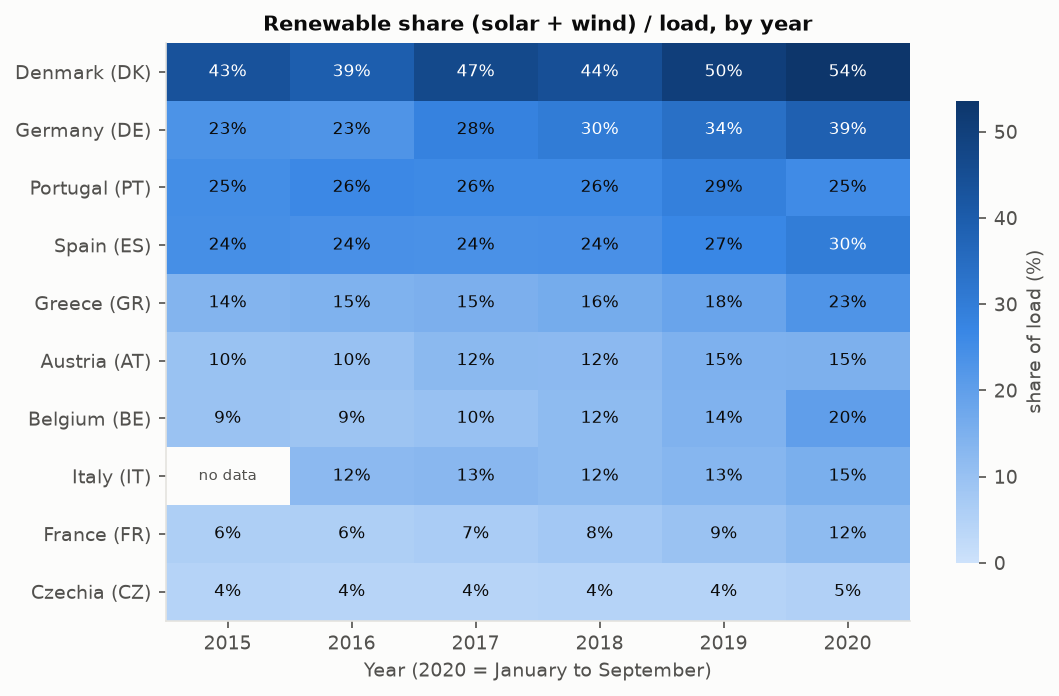
\includegraphics[width=0.75\textwidth]{1_share_by_year.png}
\caption{Renewable share (solar + wind) / load by country and year (Hive)}\label{fig:share}
\end{figure}
Denmark had the highest share in every year, from 43.4\% in 2015 to 50.4\% in 2019 and 53.6\% in January--September 2020 (Figure~\ref{fig:share}). Nearly all of it is wind: 1,819 MW of wind against 111 MW of solar on average in 2019. Germany, Portugal and Spain hold places 2 to 4 in every year, and Czechia is last at 4 to 5\%. France is ninth because most of its electricity is nuclear, which this share does not count. Germany grew the most, from 23.4\% to 33.8\% between 2015 and 2019, as its average wind output rose from 8,810 to 14,133 MW while load stayed near 55,000 MW. Every country except Czechia had a higher share in 2019 than in its first year. The daily series from Pig (Figure~\ref{fig:pig}) shows how much this moves within a year; on 2020-05-16 Danish wind and solar produced 131\% of Danish load, and the surplus was exported.

\begin{figure}[H]
\centering
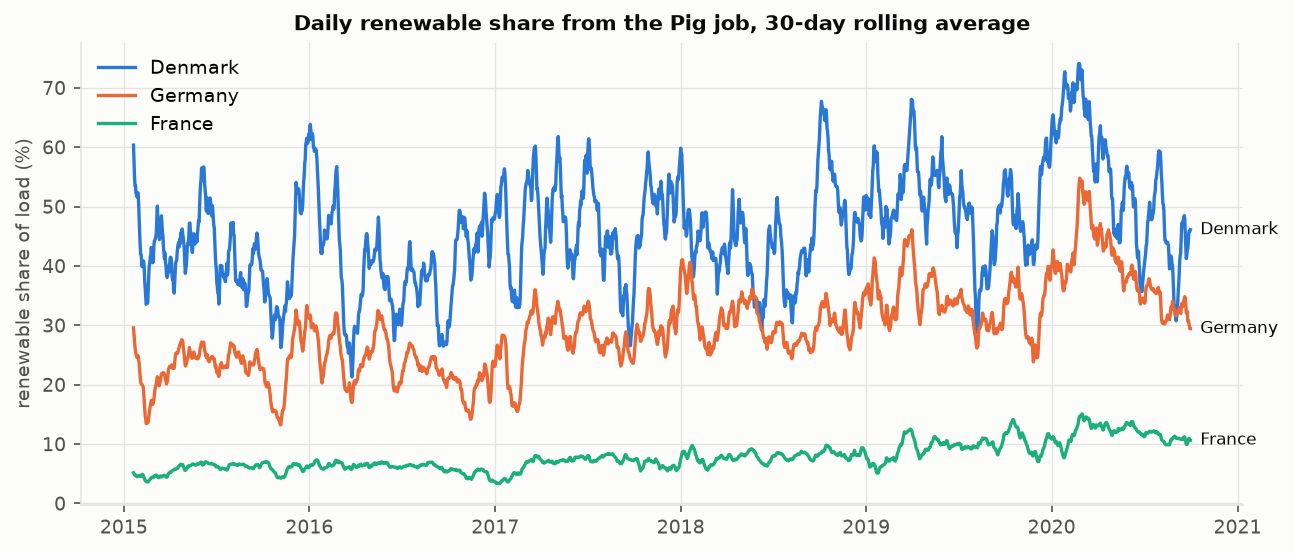
\includegraphics[width=0.8\textwidth]{6_pig_daily_share.png}
\caption{Daily renewable share, 30-day rolling average (Pig)}\label{fig:pig}
\end{figure}

\section{Q2: Daily load curve in summer and winter}
\begin{figure}[H]
\centering
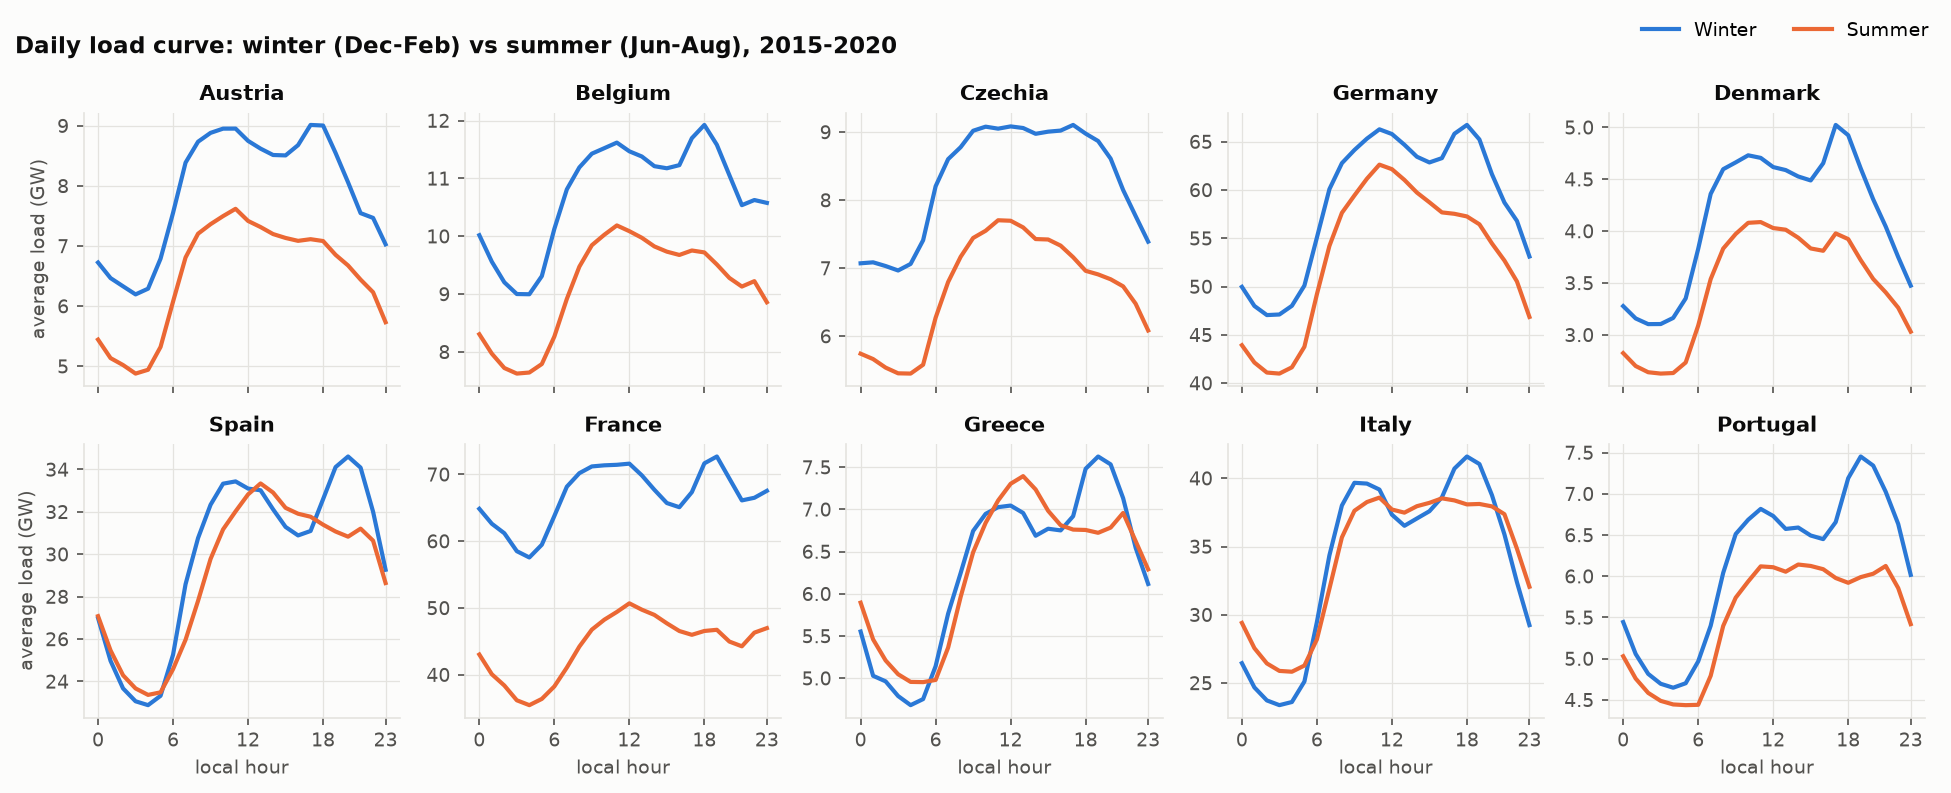
\includegraphics[width=\textwidth]{2_load_curve_summer_winter.png}
\caption{Average load by local hour, winter (Dec--Feb) and summer (Jun--Aug) (Hive)}\label{fig:curve}
\end{figure}
In every country load is lowest between 02:00 and 05:00 and rises steeply from 06:00 (Figure~\ref{fig:curve}). Winter curves have a late-morning peak and a second, usually higher, evening peak between 17:00 (Austria, Czechia, Denmark) and 20:00 (Spain), when it is dark and people are at home. Summer curves have one broad midday peak. France uses 34\% less electricity in summer than in winter, the largest gap, because many French homes are heated electrically. Spain, Greece and Italy use about the same in both seasons, since air conditioning makes up for the lower heating load.

\section{Q3: Wind peaks and demand}
\begin{figure}[H]
\centering
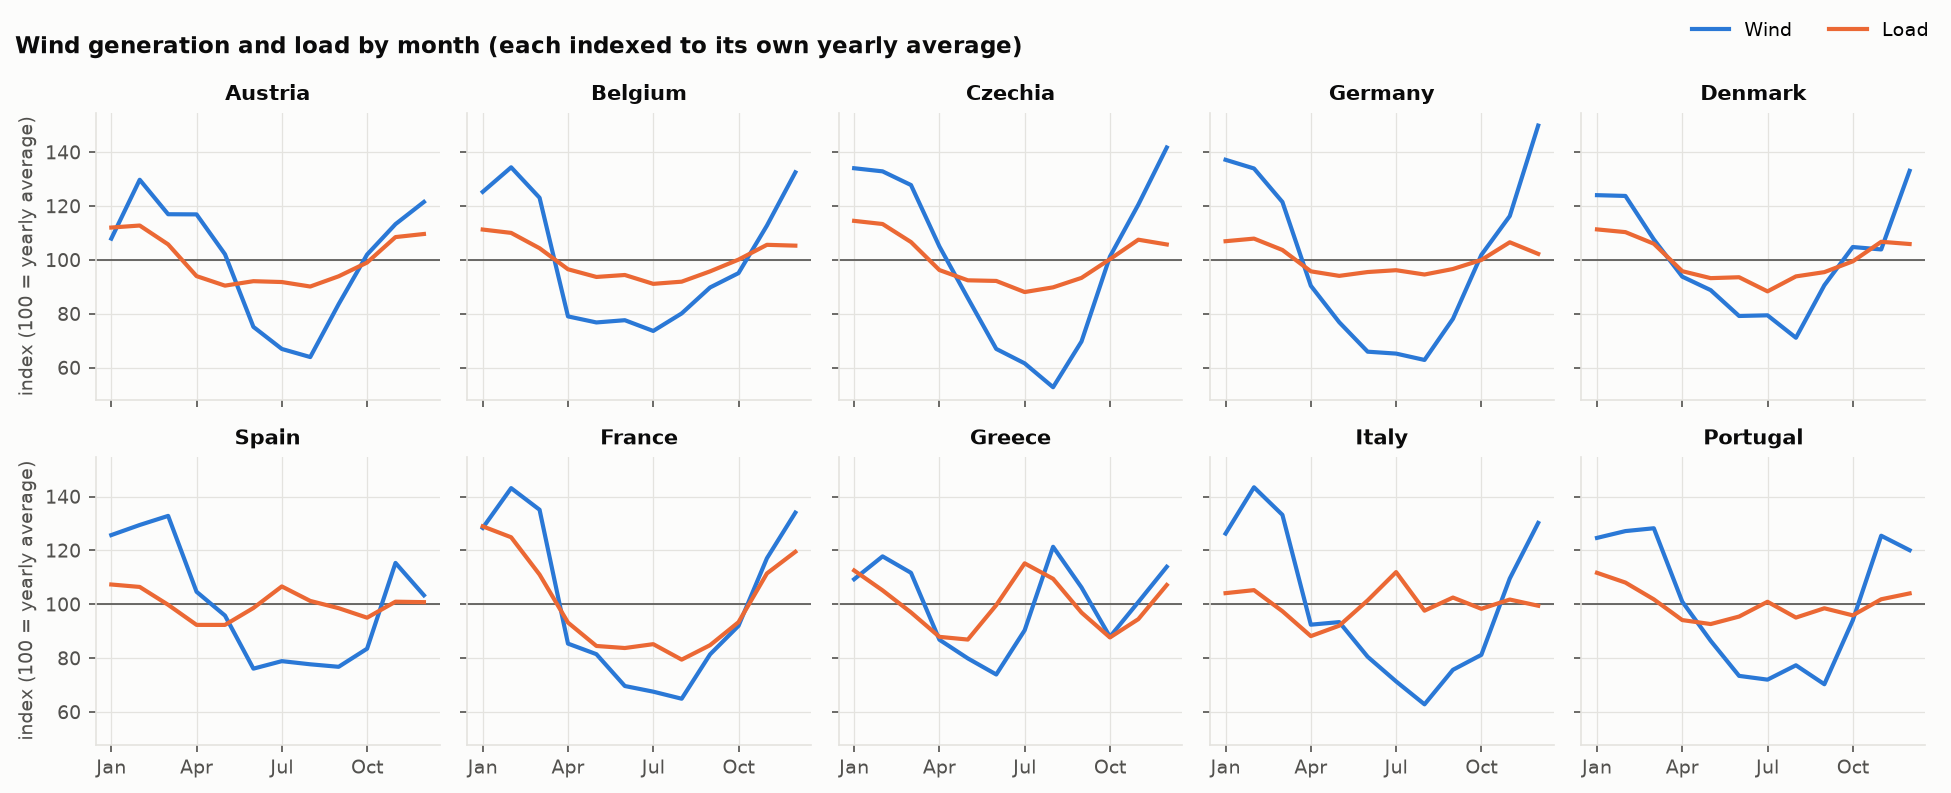
\includegraphics[width=\textwidth]{3a_wind_vs_load_by_month.png}
\caption{Wind and load by month, each indexed to its yearly average (Hive)}\label{fig:windm}
\end{figure}
By season, wind and demand line up. In nine of the ten countries wind is strongest between December and March, in all ten it is weakest between June and September, and the windiest month produces 1.6 to 2.7 times as much as the calmest. Load is also highest in winter, and the twelve monthly averages of wind and load correlate at 0.87 to 0.96 in Belgium, Czechia, Germany, Denmark and France (Figure~\ref{fig:windm}). Greece is the exception: its wind peaks in August, which matches its summer air-conditioning load. Within a day the match is poor (Figure~\ref{fig:windh}). In most countries wind is weakest at 09:00--10:00 and strongest in the late evening or at night, while load peaks around midday; the hourly profiles correlate negatively in seven countries, down to $-0.75$ in Czechia. Only Denmark and Italy have wind peaking in the afternoon, near their evening load peak.

\begin{figure}[H]
\centering
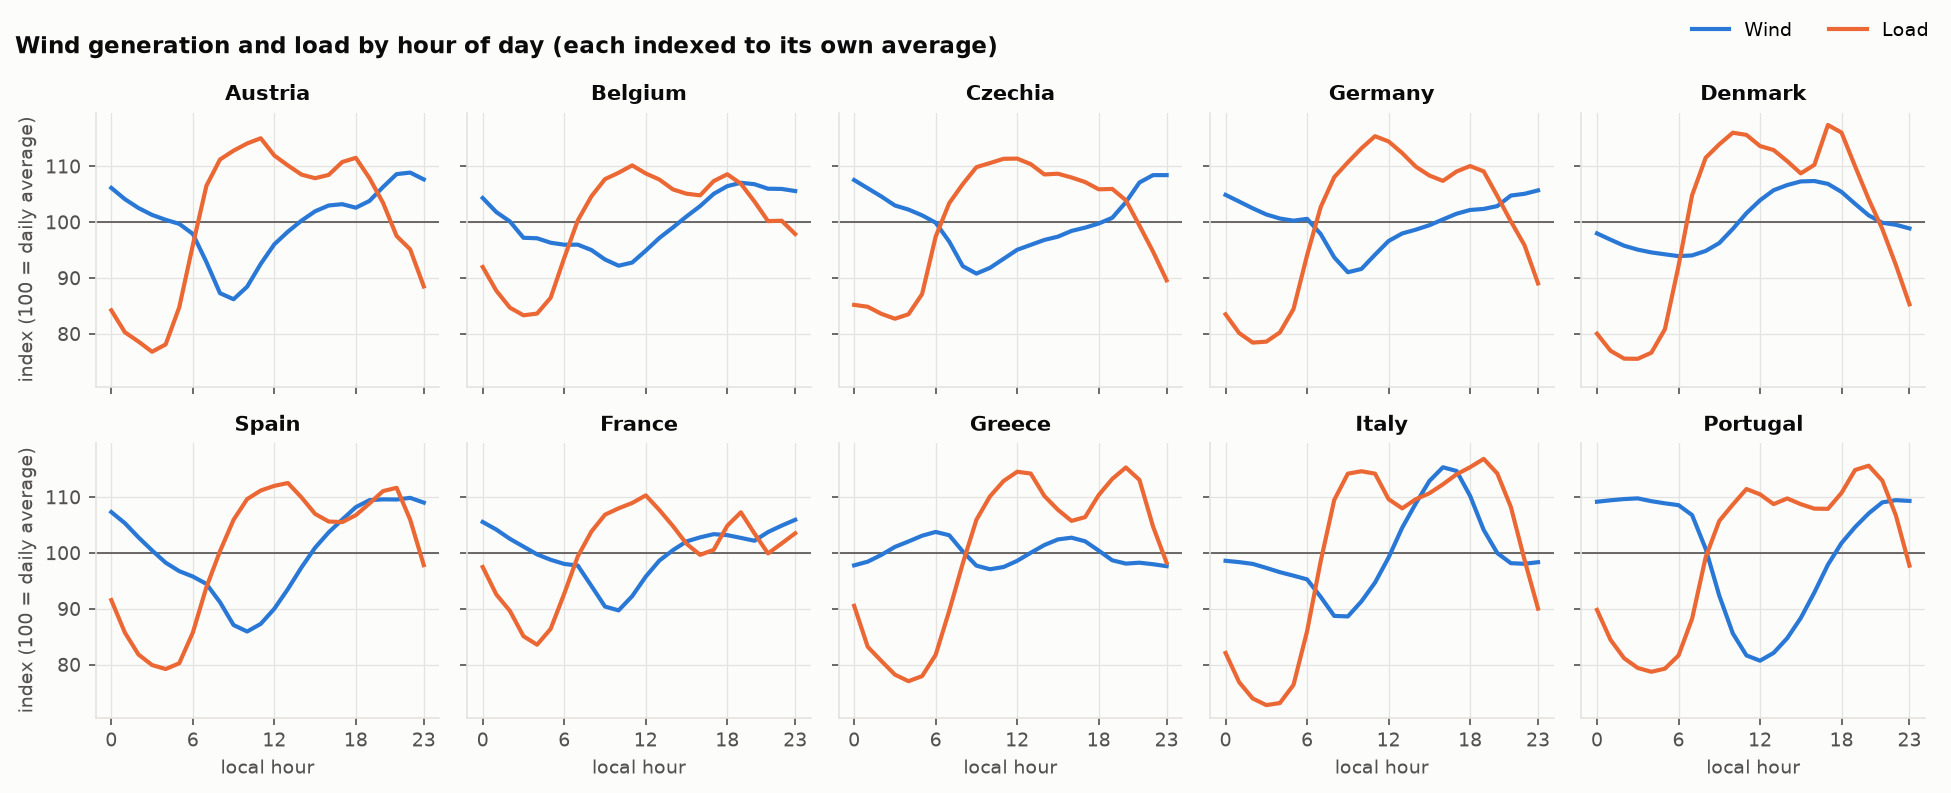
\includegraphics[width=\textwidth]{3b_wind_vs_load_by_hour.png}
\caption{Wind and load by local hour, each indexed to its average (Hive)}\label{fig:windh}
\end{figure}

\section{Q4: Hours with the largest load changes}
\begin{figure}[H]
\centering
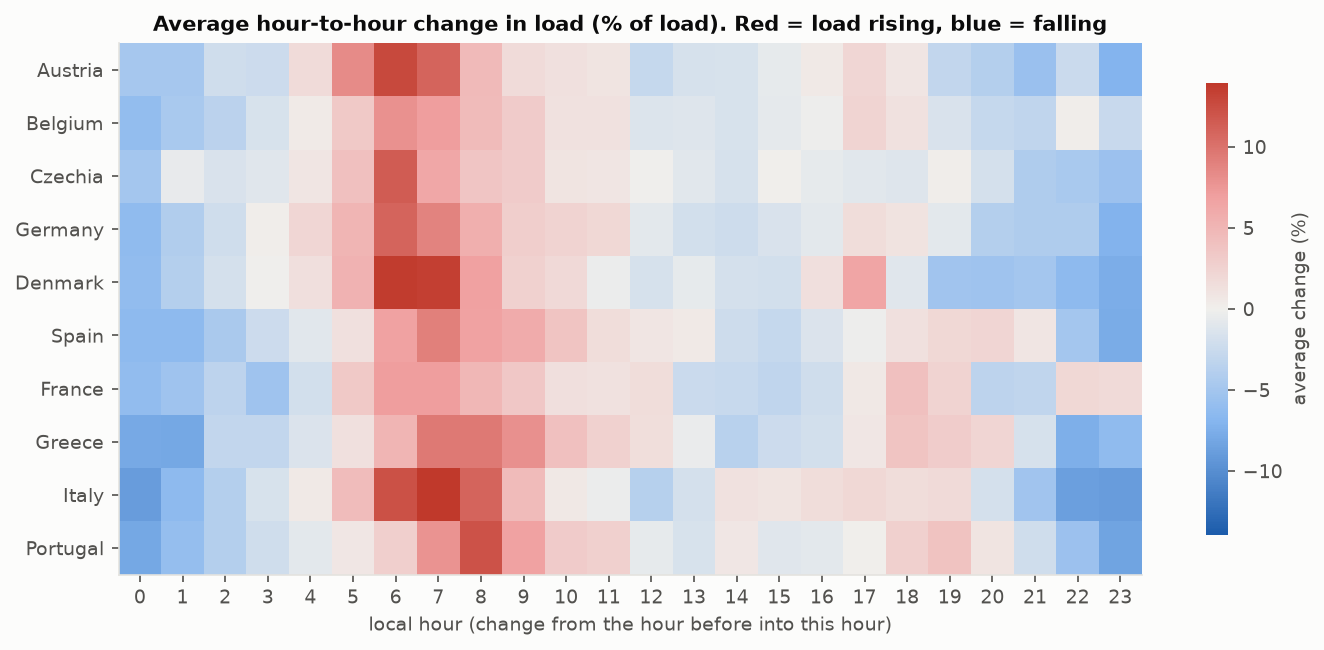
\includegraphics[width=0.85\textwidth]{4a_load_change_by_hour.png}
\caption{Average hour-to-hour change in load, in percent (Hive, LAG)}\label{fig:change}
\end{figure}
The largest changes are the morning ramp. In every country the largest average rise is into 06:00, 07:00 or 08:00 local time: +13.9\% into 07:00 in Italy, +13.6\% into 06:00 in Denmark and +10.9\% in Germany (Figure~\ref{fig:change}). The largest average drops, of 5.5 to 8.9\%, come in the late evening. In megawatts, 19 of the 20 biggest rises are German, 18 of them into 06:00 and 16 on a Monday, when industry starts after the weekend; the largest was +10,957 MW (+20.1\%) on 2015-09-22 (Figure~\ref{fig:top}).

\begin{figure}[H]
\centering
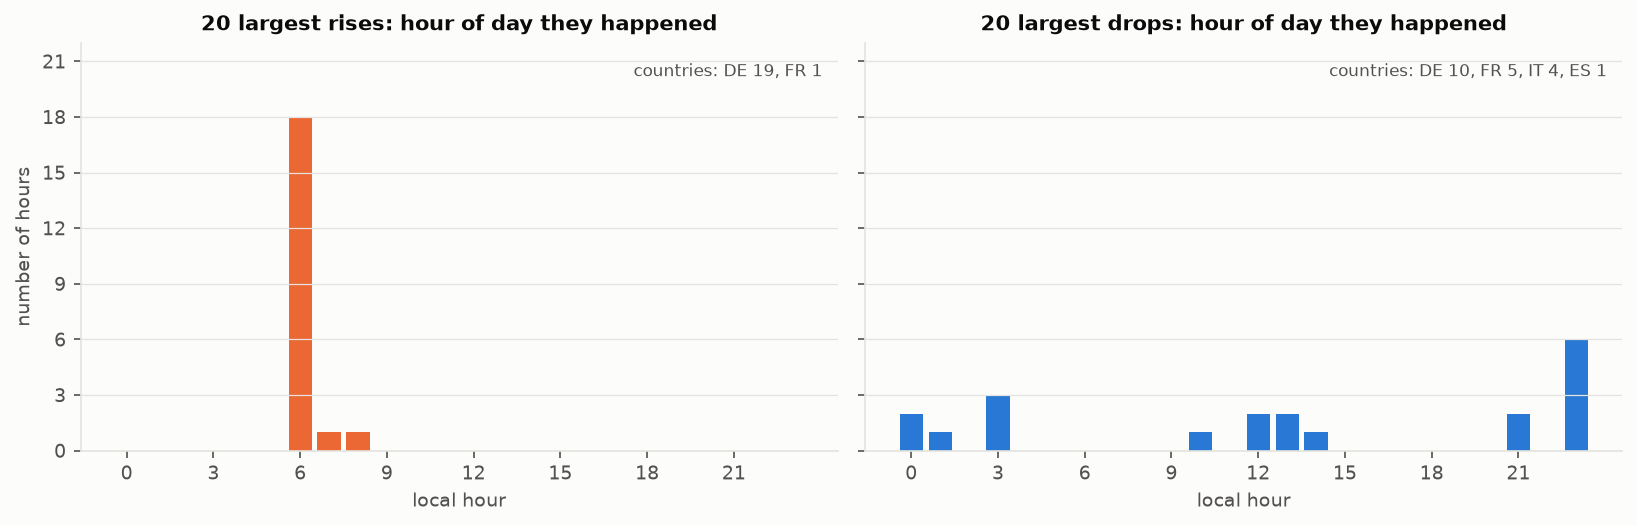
\includegraphics[width=0.85\textwidth]{4b_top_load_changes_by_hour.png}
\caption{Local hour of the 20 largest rises and drops in load (Hive, LAG)}\label{fig:top}
\end{figure}

\section{Q5: Solar generation and load}
\begin{figure}[H]
\centering
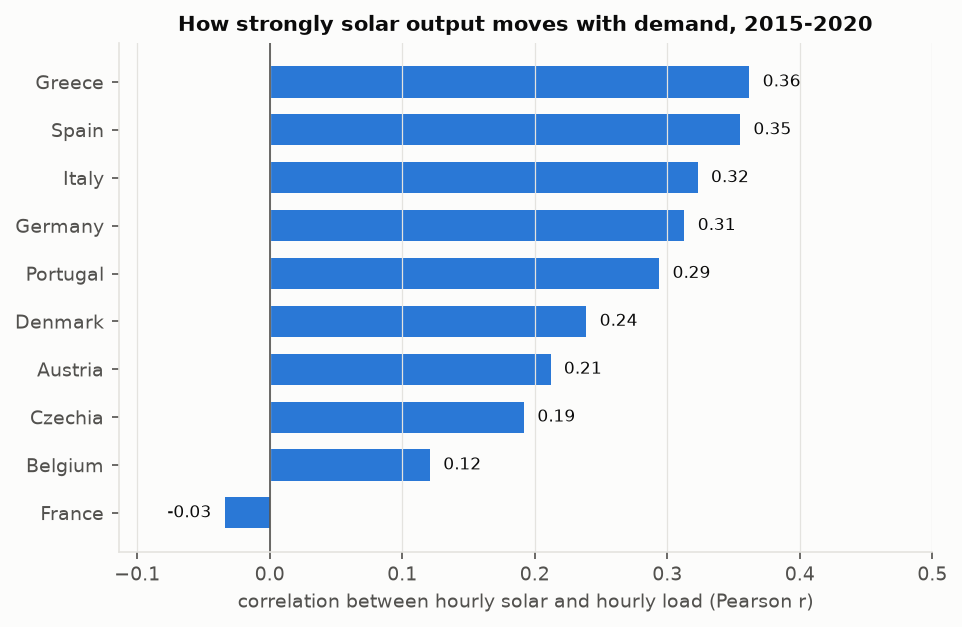
\includegraphics[width=0.6\textwidth]{5b_correlation_solar_load.png}
\caption{Correlation of hourly solar generation and load, 2015--2020 (Hive)}\label{fig:corr}
\end{figure}
The relationship is weak. The correlation of hourly solar output and load ranges from 0.12 (Belgium) to 0.36 (Greece) and is slightly negative in France ($-0.03$) (Figure~\ref{fig:corr}). Solar is zero at night and low in winter, while load is high on dark winter evenings, so the two often move apart; France, with its winter peak, shows this most. The German scatter plot (Figure~\ref{fig:scatter}) has a band at zero solar for the night hours and two clouds in daylight, which are working days (64.7 GW average load in sunny hours) and weekends (50.3 GW). In summer alone, when load peaks at midday with the sun, the correlation rises to between 0.43 and 0.64.

\begin{figure}[H]
\centering
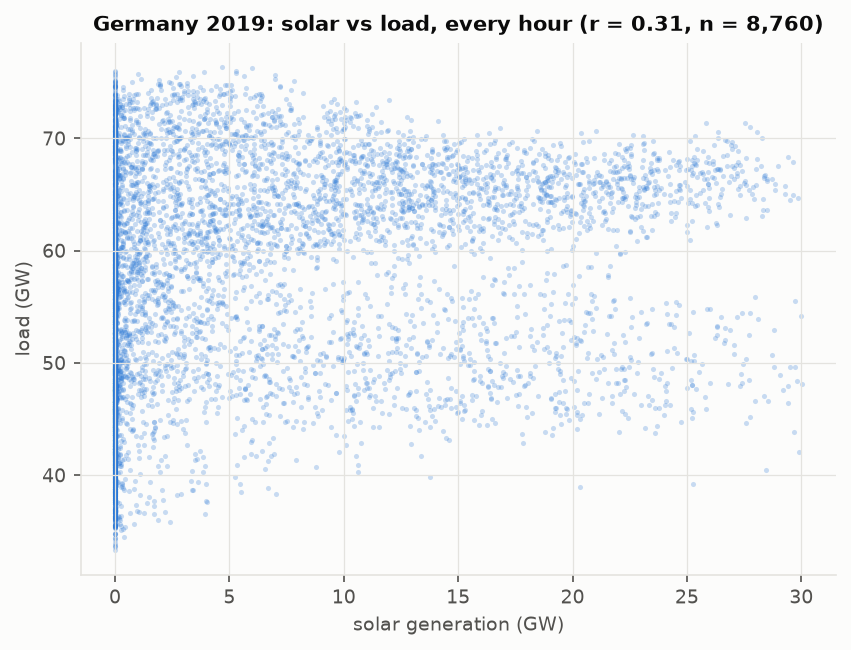
\includegraphics[width=0.55\textwidth]{5a_scatter_solar_load_DE_2019.png}
\caption{Germany 2019: hourly solar generation against load (Hive)}\label{fig:scatter}
\end{figure}

\section{Scale test}
The same jobs were run on the 2019 sample, the full file (with 128 MB and 32 MB blocks) and a five-fold copy of the full file (Table~\ref{tab:scale}).

\begin{table}[H]
\centering\small
\caption{Scale test (3 reducers, combiner on)}\label{tab:scale}
\footnotesize
\begin{tabularx}{\textwidth}{lXrrr}
\toprule
Job & Data & Map tasks & Input records & Time (s)\\
\midrule
MR Job A & sample (9.4 MB) & 1 & 262,011 & 22.6\\
MR Job A & full (52.9 MB) & 1 & 1,480,855 & 23.3\\
MR Job A & full, 32 MB blocks & 2 & 1,480,855 & 28.4\\
MR Job A & full $\times$5 (264.5 MB) & 2 & 7,404,275 & 28.6\\
MR Job B & full $\times$5 (264.5 MB) & 2 & 7,404,275 & 36.6\\
Pig script (13 jobs) & sample / full & & & 313 / 308\\
Hive GROUP BY (1 job) & sample / full / $\times$5 & & & 45 / 37 / 48\\
Hive join (3 jobs) & sample / full / $\times$5 & & & 108 / 98 / 124\\
\bottomrule
\end{tabularx}
\end{table}

Time grew far more slowly than the data. With 28 times the records of the sample, Job A took 27\% longer. On one laptop the fixed cost of starting YARN containers (around 20 seconds per job) outweighs the work of reading tens of megabytes, which is also why the multi-job Pig script and Hive join take longest and why the 32 MB-block copy, with two map tasks competing for the same machine, was slower than one task. The counters, on the other hand, scaled exactly: the five-fold file gave five times the input records and identical averages, which doubles as a correctness check. In Job B on that file the combiner processed more records than the map output (7,407,734 against 7,404,275), because it ran again when the spill files were merged.

\section{Limitations}
The share counts only solar and wind; hydro power, large in Austria, Spain and Portugal, is left out. A daily share above 100\% reflects exports, not a grid running on renewables alone. Correlation captures only straight-line relationships. The year 2020 covers nine months and includes the COVID lockdowns, and Italy has no 2015 data. The cleaning rules remove clear errors but may miss smaller ones. Finally, all timings come from one laptop and say little about speed on a real cluster.

% ==========================================================================
\chapter{Problems Faced}\label{ch:problems}
\begin{enumerate}
\item \textbf{No SSH to localhost.} \texttt{start-dfs.sh} logs in to each worker over SSH, which is off on our Macs. We start each daemon with \texttt{hdfs --daemon start} and \texttt{yarn --daemon start} instead.
\item \textbf{YARN disk check.} The disk was 93\% full and YARN marks a node unhealthy above 90\%, so no job could run until we raised the limit.
\item \textbf{Missing library in YARN tasks.} Pig 0.18 and Hive 4.2.1 still need commons-collections 3, which Hadoop 3.4 no longer ships. Adding it to the local classpath fixed the client but not the map tasks; it had to be shipped with each job (\texttt{pig.additional.jars} for Pig, \texttt{ADD JAR} for Hive).
\item \textbf{Hive setup.} The Derby driver class moved in Derby 10.17; beeline would not start on Apple Silicon because of an old native library; and Hive 4 has no \texttt{hive} shell, so we used embedded \texttt{beeline}.
\item \textbf{Managed tables became external.} Hive 4 silently turns non-transactional managed tables into external ones (\texttt{TRANSLATED\_TO\_EXTERNAL}). We disabled this with \texttt{metastore.metadata.transformer.class}; our first attempt used a wrong property name, found by searching the Hive metastore jar.
\item \textbf{Map join failure.} Hive's automatic map join starts a separate local process that did not inherit our settings and failed. We switched to reduce-side joins with \texttt{hive.auto.convert.join=false}.
\item \textbf{Reducer count.} Our first job read \texttt{mapreduce.job.reduces} with a default of 3, but Hadoop already sets it to 1, so the partitioner never had work. The counter ``Launched reduce tasks=1'' showed the bug; we switched to our own setting.
\item \textbf{Bad source data.} Unrealistic results from Pig and Hive led us to 70 faulty readings, which forced three full re-runs of the pipeline (Section~3.4).
\end{enumerate}

% ==========================================================================
\chapter{Conclusion}\label{ch:concl}

\section{Conclusion}
We set up a pseudo-distributed Hadoop cluster with Pig and Hive and used it to analyse six years of hourly electricity data for ten countries. All required elements were implemented: HDFS directories, a non-default block size, a replication change and \texttt{fsck}; two Java MapReduce jobs with a combiner, a partitioner and counters; a Pig script with ten operators; Hive external, managed, partitioned, Parquet and ORC tables with a join, grouping and window functions; nine charts; and a scale test. MapReduce, Hive and an independent pandas check gave the same numbers.

Denmark leads on renewable share and Germany grew fastest; wind matches demand by season but not by hour; the morning ramp is the most demanding hour for the grid; and solar is only weakly tied to load outside summer. The most useful lesson was that the results themselves exposed errors in the data, which a quick look at the raw file would have missed.

\section{Future scope}
\begin{itemize}
\item Add data from 2021 onwards to cover the 2022 energy crisis, and hydro generation for a fuller renewable share.
\item Include the electricity prices in the same OPSD file, to see how prices move with wind and solar output.
\item Run the pipeline on a multi-node cluster to show replication, data locality and real parallel speed-up, and compare with Spark or Hive on Tez.
\end{itemize}

% ==========================================================================
\begin{thebibliography}{99}
\addcontentsline{toc}{chapter}{References}

\bibitem{opsd2020} Open Power System Data, ``Data Package Time series,'' Version 2020-10-06, 2020. [Online]. Available: \url{https://doi.org/10.25832/time_series/2020-10-06}

\bibitem{wiese2019} F. Wiese, I. Schlecht, W.-D. Bunke, C. Gerbaulet, L. Hirth, M. Jahn, F. Kunz, C. Lorenz, J. M\"uhlenpfordt, J. Reimann, and W.-P. Schill, ``Open Power System Data -- Frictionless data for electricity system modelling,'' \emph{Applied Energy}, vol. 236, pp. 401--409, 2019, doi: 10.1016/j.apenergy.2018.11.097.

\bibitem{entsoe} ENTSO-E, ``Transparency Platform,'' European Network of Transmission System Operators for Electricity. [Online]. Available: \url{https://transparency.entsoe.eu/}

\bibitem{gfs2003} S. Ghemawat, H. Gobioff, and S.-T. Leung, ``The Google file system,'' in \emph{Proc. 19th ACM Symposium on Operating Systems Principles (SOSP)}, 2003, pp. 29--43.

\bibitem{hdfs2010} K. Shvachko, H. Kuang, S. Radia, and R. Chansler, ``The Hadoop distributed file system,'' in \emph{Proc. IEEE 26th Symposium on Mass Storage Systems and Technologies (MSST)}, 2010, pp. 1--10.

\bibitem{dean2008} J. Dean and S. Ghemawat, ``MapReduce: Simplified data processing on large clusters,'' \emph{Communications of the ACM}, vol. 51, no. 1, pp. 107--113, 2008.

\bibitem{lin2010} J. Lin and C. Dyer, \emph{Data-Intensive Text Processing with MapReduce}. Morgan \& Claypool, 2010.

\bibitem{yarn2013} V. K. Vavilapalli et al., ``Apache Hadoop YARN: Yet another resource negotiator,'' in \emph{Proc. 4th ACM Symposium on Cloud Computing (SoCC)}, 2013, Article 5.

\bibitem{white2015} T. White, \emph{Hadoop: The Definitive Guide}, 4th ed. O'Reilly Media, 2015.

\bibitem{olston2008} C. Olston, B. Reed, U. Srivastava, R. Kumar, and A. Tomkins, ``Pig Latin: A not-so-foreign language for data processing,'' in \emph{Proc. ACM SIGMOD International Conference on Management of Data}, 2008, pp. 1099--1110.

\bibitem{thusoo2009} A. Thusoo, J. S. Sarma, N. Jain, Z. Shao, P. Chakka, S. Anthony, H. Liu, P. Wyckoff, and R. Murthy, ``Hive: A warehousing solution over a map-reduce framework,'' \emph{Proc. VLDB Endowment}, vol. 2, no. 2, pp. 1626--1629, 2009.

\bibitem{huai2014} Y. Huai et al., ``Major technical advancements in Apache Hive,'' in \emph{Proc. ACM SIGMOD International Conference on Management of Data}, 2014, pp. 1235--1246.

\bibitem{melnik2010} S. Melnik, A. Gubarev, J. J. Long, G. Romer, S. Shivakumar, M. Tolton, and T. Vassilakis, ``Dremel: Interactive analysis of web-scale datasets,'' \emph{Proc. VLDB Endowment}, vol. 3, no. 1--2, pp. 330--339, 2010.

\bibitem{parquet} Apache Software Foundation, ``Apache Parquet documentation.'' [Online]. Available: \url{https://parquet.apache.org/docs/}

\bibitem{hadoopdocs} Apache Software Foundation, ``Apache Hadoop 3.4.2 documentation.'' [Online]. Available: \url{https://hadoop.apache.org/docs/r3.4.2/}

\bibitem{hunter2007} J. D. Hunter, ``Matplotlib: A 2D graphics environment,'' \emph{Computing in Science \& Engineering}, vol. 9, no. 3, pp. 90--95, 2007.

\bibitem{repo} K. Mungase, S. Deshmukh, V. Bhosale, and \todo{[Sneh full name]}, ``P11-Energy: Electricity load and renewable energy in Europe with Hadoop,'' GitHub repository, 2026. [Online]. Available: \url{https://github.com/krishmungase/P11-Energy}

\end{thebibliography}

\end{document}
